\documentclass[12pt,a4paper]{article}
\usepackage{fontspec}
\setmainfont{Times New Roman}
\setmonofont[Scale=0.85]{Consolas}
\usepackage[a4paper,left=28mm,right=25mm,top=29mm,bottom=25mm,headsep=7mm]{geometry}
\usepackage{graphicx,pdfpages,tabularx,booktabs,array,xcolor,fancyhdr}
\usepackage[hidelinks]{hyperref}
\usepackage{enumitem}
\setlist{nosep,leftmargin=1.6em}
\setlength{\parskip}{4pt}
\setlength{\parindent}{1em}
\linespread{1.18}
\pagestyle{fancy}
\fancyhf{}
\fancyhead[C]{\thepage}
\renewcommand{\headrulewidth}{0pt}
\setlength{\headheight}{16pt}
\newcommand{\orig}[1]{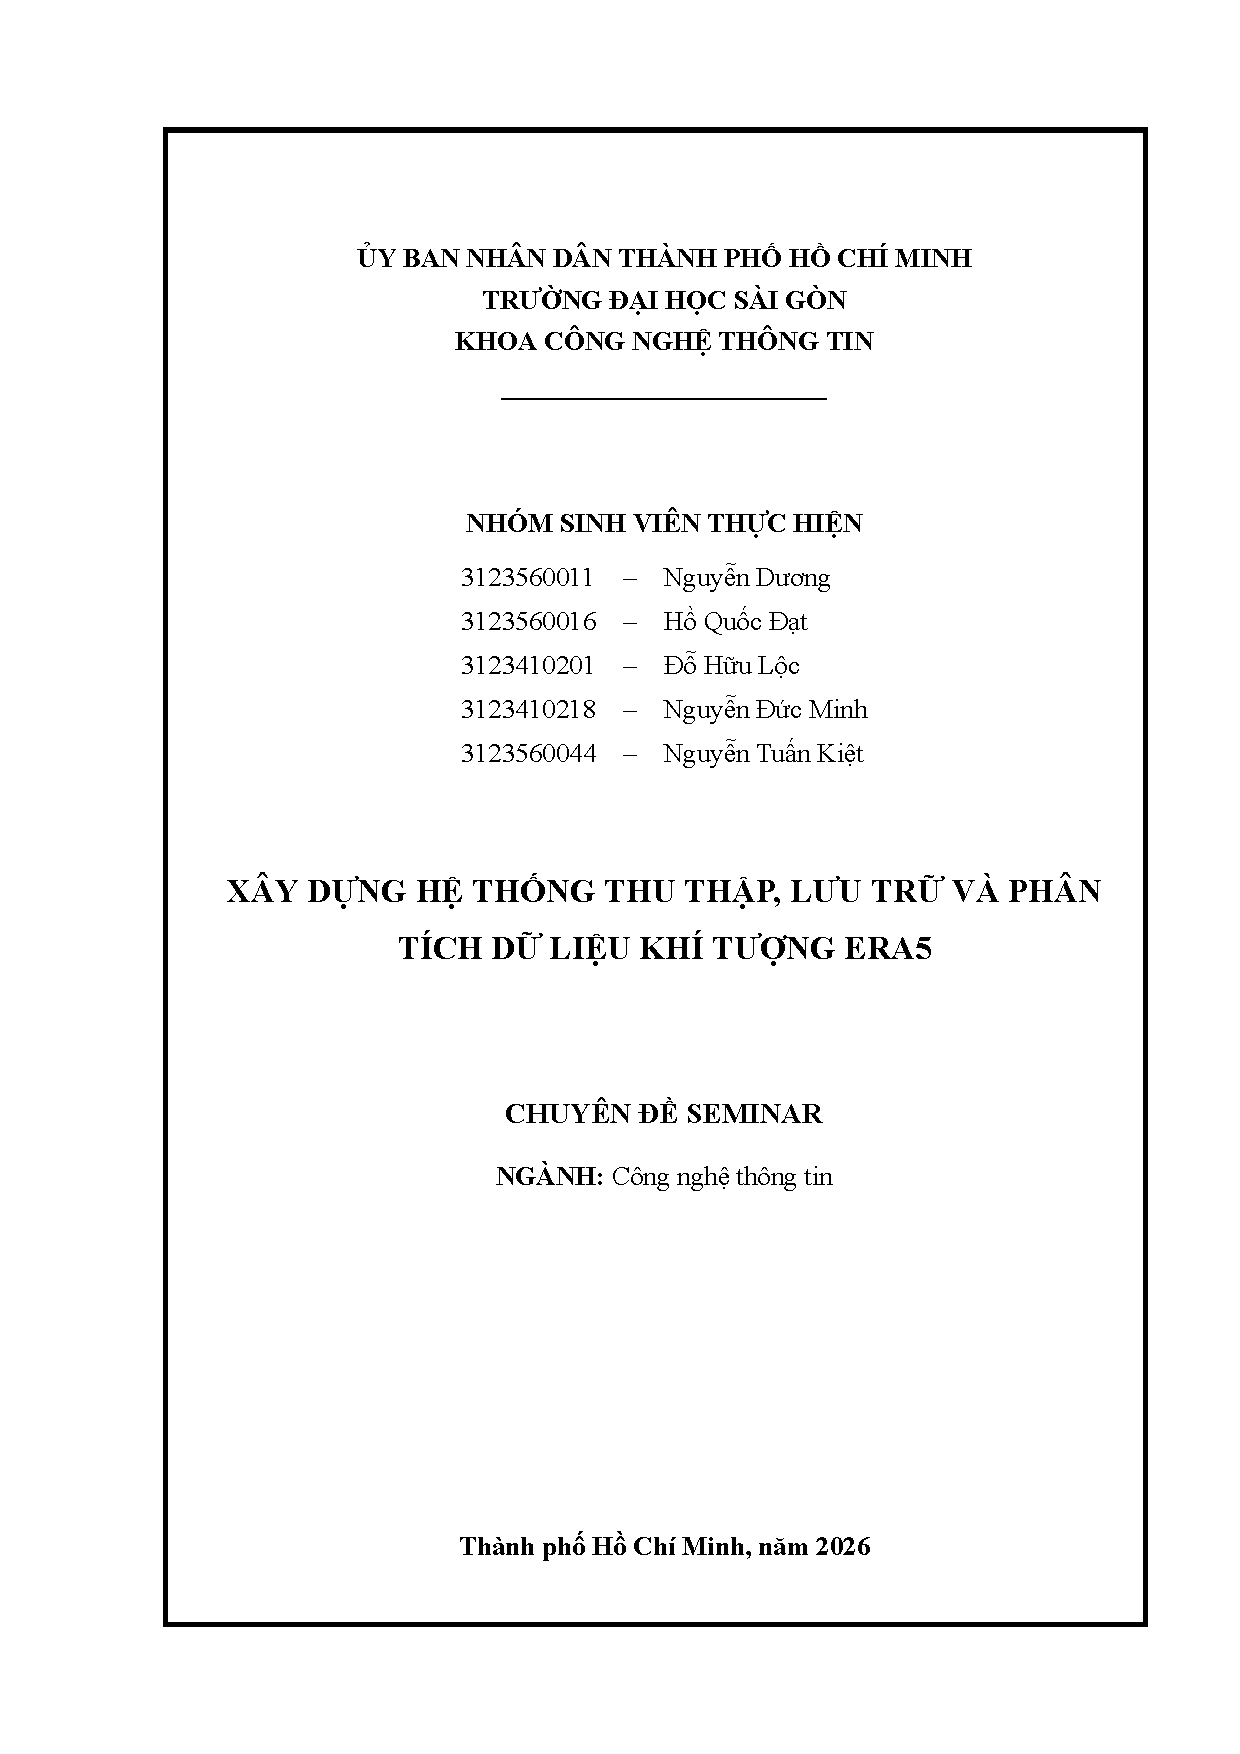
\includepdf[pages={#1},pagecommand={\thispagestyle{empty}}]{original.pdf}}
\newcommand{\pg}[1]{\newpage\pagenumbering{arabic}\setcounter{page}{#1}\thispagestyle{fancy}}
\newcommand{\heading}[1]{\par\medskip\noindent\textbf{#1}\par\nopagebreak}
\newcommand{\chaptertitle}[1]{\begin{center}\large\bfseries #1\end{center}}
\newcommand{\code}[1]{\texttt{#1}}
\newcommand{\fig}[4]{\par\noindent\begin{minipage}{\linewidth}\centering
\includegraphics[width=#3\linewidth,height=#4mm,keepaspectratio]{screenshots/#1.png}\par
\small #2\end{minipage}\par\smallskip}
\newcommand{\captext}[1]{\begin{center}\small #1\end{center}}
\newcommand{\pair}[2]{#1 & #2\\\addlinespace[4pt]}
\newcommand{\nodebox}[1]{\fcolorbox{black!28}{black!4}{\begin{minipage}{0.88\linewidth}\centering #1\end{minipage}}}
\newcommand{\arrowline}{\par\centering $\downarrow$\par}
\newcommand{\listrow}[2]{\noindent #1\dotfill #2\par}
\begin{document}
\orig{1-2}
\newpage\pagenumbering{roman}\setcounter{page}{1}
\chaptertitle{LỜI CAM ĐOAN}
Chúng tôi, nhóm sinh viên thực hiện chuyên đề seminar dưới sự hướng dẫn của giảng viên Phạm Thế Bảo, gồm các thành viên sau.

\begin{center}
\begin{tabular}{ll}
3123560011 & Nguyễn Dương\\
3123560016 & Hồ Quốc Đạt\\
3123410201 & Đỗ Hữu Lộc\\
3123410218 & Nguyễn Đức Minh\\
3123560044 & Nguyễn Tuấn Kiệt
\end{tabular}
\end{center}

\bigskip
\begin{flushright}
Thành phố Hồ Chí Minh, ngày \ldots\ tháng \ldots\ năm 2026\\
\textbf{Đại diện nhóm thực hiện}\\[2.5em]
\textit{(Ký và ghi rõ họ tên)}
\end{flushright}
\newpage\pagenumbering{roman}\setcounter{page}{2}
\chaptertitle{LỜI CẢM ƠN}
Trước hết, nhóm thực hiện xin gửi lời cảm ơn chân thành đến GV Phạm Thế Bảo đã định hướng chuyên môn và góp ý trong suốt quá trình thực hiện chuyên đề seminar.

Nhóm thực hiện cũng xin trân trọng cảm ơn quý Thầy, Cô Khoa Công nghệ Thông tin, Trường Đại học Sài Gòn đã trang bị kiến thức nền tảng về kỹ thuật phần mềm, cơ sở dữ liệu và phân tích dữ liệu để nhóm triển khai sản phẩm.

Cuối cùng, nhóm xin cảm ơn gia đình, bạn bè và các bạn cùng lớp đã hỗ trợ, góp ý kiểm thử và động viên nhóm trong quá trình hoàn thành chuyên đề.
\orig{5-6}
\newpage\pagenumbering{roman}\setcounter{page}{5}
\listrow{4.3. Kết quả phân tích và trực quan hóa dữ liệu thực}{28}
\listrow{4.4. Kết quả kiểm thử tự động và phân tích lỗi}{33}
\listrow{4.5. Các lỗi vận hành và những giới hạn chưa giải quyết}{35}
\medskip
\listrow{\textbf{KẾT LUẬN VÀ KHUYẾN NGHỊ}}{36}
\listrow{Kết quả đạt được}{36}
\listrow{Hạn chế và các vấn đề chưa hoàn thành}{36}
\listrow{Hướng phát triển tiếp theo}{36}
\medskip
\listrow{\textbf{TÀI LIỆU THAM KHẢO}}{37}
\medskip
\listrow{\textbf{PHỤ LỤC}}{39}
\listrow{Phụ lục P.1. Danh sách đầy đủ HTTP API Endpoints}{39}
\listrow{Phụ lục P.2. Cấu trúc mã nguồn dự án}{40}
\listrow{Phụ lục P.3. Hướng dẫn cài đặt, cấu hình mẫu và tái tạo kết quả}{41}
\orig{8-9}
\newpage\pagenumbering{roman}\setcounter{page}{8}
\chaptertitle{DANH MỤC CÁC BIỂU, BẢNG}
\listrow{1.1. So sánh hai bộ dữ liệu ERA5 và ERA5-Land}{7}
\listrow{1.2. Biến khí tượng, đơn vị lưu trữ và đơn vị hiển thị}{8}
\listrow{2.1. Tổng hợp các nhóm yêu cầu chức năng}{13}
\listrow{2.2. Phân rã trách nhiệm các module chính}{15}
\listrow{4.1. Phiên bản môi trường và thư viện cốt lõi}{27}
\listrow{4.2. Tổng hợp sáu biến nguồn ERA5-Land tại lưới Hà Nội}{29}
\listrow{4.3. Thống kê tác vụ trong kho dùng để đối chiếu}{29}
\listrow{4.4. Tổng hợp nhiệt độ 2 m theo ngày tại lưới Hà Nội}{30}
\listrow{4.5. Phân nhóm các tệp kiểm thử tự động}{34}
\listrow{P1.1. Danh sách các HTTP API endpoint của hệ thống}{39}
\newpage\pagenumbering{roman}\setcounter{page}{9}
\chaptertitle{DANH MỤC HÌNH ẢNH, SƠ ĐỒ}
\listrow{2.1. Kiến trúc tổng thể các tầng xử lý và luồng tích hợp}{14}
\listrow{2.2. Cấu trúc các bảng SQLite và khóa liên kết}{16}
\listrow{2.3. Vòng đời yêu cầu HTTP có xác thực}{17}
\listrow{2.4. Sơ đồ trạng thái và vòng đời tác vụ thu thập}{17}
\listrow{2.5. Luồng đồng bộ và điều kiện cập nhật mốc}{18}
\listrow{3.1. Kiểm tra độ phủ và tải bổ sung ở API tương thích}{21}
\listrow{3.2. Cổng đăng nhập và đăng ký}{23}
\listrow{3.3. Thu thập dữ liệu và theo dõi tác vụ}{24}
\listrow{3.4. Chi tiết bộ dữ liệu trong kho}{24}
\listrow{3.5. Luồng điều phối công cụ của ARE}{25}
\listrow{3.6. ARE truy vấn thống kê trên dữ liệu đã lưu}{26}
\listrow{3.7. Tổng quan quản trị và lịch sử thu thập}{26}
\listrow{4.1. Nhiệt độ 2 m và điểm sương theo giờ}{30}
\listrow{4.2. Lượng mưa theo giờ}{31}
\listrow{4.3. Bức xạ mặt trời hướng xuống theo giờ}{31}
\listrow{4.4. Tốc độ gió 10 m theo giờ}{32}
\listrow{4.5. Nhiệt độ trung bình và khoảng min–max theo ngày}{32}
\listrow{4.6. Biểu đồ nhiệt độ và điểm sương trên Dashboard}{33}
\listrow{P.1. Tài liệu API tương tác qua Swagger UI}{40}

\orig{12-14}
\pg{4}
\begin{itemize}
\item Phân tích và thiết kế hướng miền kết hợp tách lớp. Hợp đồng dữ liệu tại \code{domain/}, provider ở \code{providers/}, nghiệp vụ ở \code{services/} và truy cập SQLite ở \code{storage/}.
\item Kiểm chứng bằng pytest, FastAPI TestClient và Streamlit AppTest. Đối chiếu dữ liệu ERA5-Land giữa tệp nguồn và SQLite. Chạy ứng dụng trong trình duyệt để ghi nhận giao diện thực tế.
\end{itemize}
\heading{6. Giả thuyết khoa học}
Việc lưu riêng các lần thu thập, lưu tọa độ lưới thực, chuẩn hóa thời gian UTC và trả độ phủ theo kỳ lịch cho phép tái sử dụng dữ liệu và diễn giải kết quả có kiểm soát. Có thể kiểm chứng giả thuyết qua so sánh giá trị sau chuẩn hóa, kiểm tra giờ thiếu và tái hiện các phép tổng hợp ở ranh giới UTC+7.
\heading{7. Những đóng góp mới}
\begin{enumerate}
\item Tổ chức luồng thu thập ERA5-Land theo điểm trên Dashboard và cung cấp các API đọc dữ liệu đã lưu cho Kho dữ liệu, Biểu đồ và ARE.
\item Lưu bộ dữ liệu theo từng lần thu thập và gắn báo cáo chất lượng. Phần thiếu được ghi nhận, còn tác vụ có thể yêu cầu hủy hợp tác và được kiểm tra khi backend khởi động lại.
\item Cô lập dữ liệu nghiệp vụ theo tài khoản. Dashboard và trang quản trị riêng dùng chung backend, với quyền truy cập quản trị được xác minh tại API.
\item Cung cấp sáu chế độ biểu đồ trên dữ liệu đã lưu và trợ lý ARE có công cụ đọc dữ liệu, chuẩn bị điều hướng, chuẩn bị bản nháp thu thập để người dùng xác nhận.
\end{enumerate}
\pg{5}
\heading{8. Cấu trúc của chuyên đề}
\begin{itemize}
\item \textbf{Chương 1. Cơ sở lý thuyết và công nghệ.} Nguồn ERA5 và ERA5-Land, đơn vị và thời gian, công thức gió, tổng hợp và thống kê.
\item \textbf{Chương 2. Phân tích yêu cầu và thiết kế hệ thống.} Tác nhân, kiến trúc, dữ liệu, xác thực, API và vòng đời tác vụ.
\item \textbf{Chương 3. Xây dựng và triển khai giải pháp.} Provider CDS, lưu trữ và kiểm soát chất lượng, giao diện, trang quản trị và ARE.
\item \textbf{Chương 4. Thực nghiệm, kết quả và đánh giá.} Đối chiếu 864 giá trị ERA5-Land, phân tích chu kỳ ngày–đêm, độ phủ, kiểm thử offline và giới hạn triển khai.
\end{itemize}
\heading{Phiên bản sử dụng để đối chiếu}
Giao diện và hướng dẫn thao tác được cập nhật theo commit \code{d25793d} trên nhánh \code{NDuong}. Kết quả kiểm thử toàn bộ ở mục 4.4 ghi theo commit \code{6033802}. Các bảng và đồ thị khí tượng dựa trên mẫu dữ liệu Hà Nội đã lưu cục bộ. Ảnh giao diện được chụp từ các dịch vụ chạy riêng trên localhost, dùng tài khoản trình diễn và bản sao kho dữ liệu. Màn hình ARE sử dụng phản hồi gọi công cụ cố định để kiểm tra tích hợp với cơ sở dữ liệu, độc lập với chất lượng trả lời của gateway mô hình trực tuyến.

\orig{17}
\pg{7}
\noindent nên yêu cầu có thể phải chờ trong hàng đợi trước khi CDS xử lý.
\captext{\textbf{Bảng 1.1.} So sánh hai bộ dữ liệu ERA5 và ERA5-Land được tích hợp}
\small
\begin{tabularx}{\linewidth}{@{}p{.23\linewidth}XX@{}}
\toprule Tiêu chí & ERA5 Single Levels & ERA5-Land Time-series\\\midrule

Mã CDS & \code{reanalysis-era5-single-levels} & \code{reanalysis-era5-land-timeseries}\\
Phạm vi & Đất liền và biển & Điểm trên đất liền\\
Lưới phân phối & 0,25° & 0,1°\\
Bước thời gian & Một giờ & Một giờ\\
Cách truy xuất & API tương thích hỗ trợ tải theo vùng với bốn cận. & Dashboard và ARE thu thập theo một cặp vĩ độ–kinh độ, yêu cầu sáu biến nguồn trong cùng lượt truy xuất.\\
Định dạng trong ứng dụng & NetCDF; vùng dài ngày có thể chia đợt & ZIP/CSV chuỗi thời gian điểm\\
\bottomrule
\end{tabularx}
\normalsize
\heading{1.2.2. Định dạng NetCDF và CSV chuỗi thời gian}
NetCDF lưu dữ liệu đa chiều cùng các trục tọa độ, thời gian và siêu dữ liệu [11]. Hệ thống dùng xarray [6] để đọc biến trên lưới và chọn nút lưới gần tọa độ yêu cầu khi lấy chuỗi một điểm. Với ERA5-Land time-series, CDS trích xuất tại một vị trí và trả các tệp CSV theo nhóm biến trong gói ZIP.
 
Hai nguồn phục vụ nhu cầu khác nhau. ERA5 phù hợp khi cần vùng có điểm lưới trên biển hoặc cần so sánh không gian. ERA5-Land time-series phù hợp khi cần chuỗi tại một điểm đất liền. Khi đánh giá kết quả, ghi rõ tọa độ yêu cầu, tọa độ lưới thực và nguồn đã chọn.

\pg{8}
\heading{1.3. Các biến khí tượng, quy ước đơn vị và xử lý thời gian}
\heading{1.3.1. Danh mục biến khí tượng hỗ trợ}
Hệ thống thu thập sáu biến nguồn và tính tốc độ, hướng gió từ hai thành phần gió 10 m. Các mã ngắn \code{t2m}, \code{d2m} và \code{tp} là tên trường có thể gặp trong tệp nguồn. Khi gọi API, có thể dùng tên chuẩn trong bảng.
\captext{\textbf{Bảng 1.2.} Danh mục các biến khí tượng, đơn vị lưu trữ và đơn vị hiển thị}
\begin{tabularx}{\linewidth}{@{}p{.54\linewidth}XXX@{}}
\toprule Tên chuẩn & Đơn vị CDS & Đơn vị lưu & Đơn vị hiển thị\\\midrule
\code{2m\_temperature} & K & K & °C\\
\code{2m\_dewpoint\_temperature} & K & K & °C\\
\code{total\_precipitation} & m & mm & mm\\
{\small \code{surface\_solar\_radiation\_downwards}} & J/m² & MJ/m² & MJ/m²\\
\code{10m\_u\_component\_of\_wind} & m/s & m/s & m/s\\
\code{10m\_v\_component\_of\_wind} & m/s & m/s & m/s\\
\code{wind\_speed} (dẫn xuất) & — & — & m/s\\
\code{wind\_direction} (dẫn xuất) & — & — & °\\
\bottomrule
\end{tabularx}
\heading{1.3.2. Công thức quy đổi đơn vị và chuẩn hóa múi giờ}
\begin{eqnarray*}
T(\mathrm{^{\circ}C}) &=& T(\mathrm K)-273{,}15 \qquad (1.1)\\
P(\mathrm{mm}) &=& 1000P(\mathrm m) \qquad (1.2)\\
E(\mathrm{MJ/m^2}) &=& E(\mathrm{J/m^2})/10^6 \qquad (1.3)\\
t_{\mathrm{VN}} &=& t_{\mathrm{UTC}}+7\ \textnormal{giờ} \qquad (1.4)
\end{eqnarray*}
Provider quy đổi lượng mưa và bức xạ từ đơn vị nguồn trước khi lưu. Tầng dịch vụ quy đổi nhiệt độ khi trả kết quả. Dấu thời gian của quan sát được lưu theo UTC và hiển thị theo UTC+7.
\orig{20-21}
\pg{11}
\heading{1.5. Các công nghệ sử dụng trong hệ thống}
Hệ thống sử dụng Python. Môi trường đối chiếu của bản báo cáo này chạy Python 3.12.10. Bảng 4.1 ghi các phiên bản thư viện đã sử dụng khi kiểm thử.
\begin{itemize}
\item \textbf{FastAPI và Pydantic.} Xây dựng API HTTP, sinh tài liệu OpenAPI và kiểm tra dữ liệu đầu vào theo schema [12].
\item \textbf{SQLite.} Lưu dữ liệu khí tượng, tác vụ và tài khoản. WAL hỗ trợ truy cập đồng thời và UPSERT cập nhật các giá trị cache trùng khóa [13].
\item \textbf{xarray, netCDF4 và pandas.} Đọc dữ liệu đa chiều từ NetCDF, xử lý bảng CSV và chuỗi thời gian [6], [14].
\item \textbf{Streamlit và Plotly.} Cung cấp Dashboard, trang quản trị và các biểu đồ tương tác [15], [16].
\item \textbf{APScheduler và pwdlib.} Lập lịch đồng bộ định kỳ và băm mật khẩu bằng Argon2id [17].
\end{itemize}
\pg{12}
\chaptertitle{CHƯƠNG 2. PHÂN TÍCH YÊU CẦU VÀ THIẾT KẾ HỆ THỐNG}
\heading{2.1. Hiện trạng bài toán và các tác nhân sử dụng}
\begin{enumerate}
\item \textbf{Người dùng Dashboard.} Đăng ký hoặc đăng nhập, tạo tác vụ thu thập, xem chất lượng bộ dữ liệu, phân tích, tải CSV và trao đổi với ARE.
\item \textbf{Quản trị viên.} Truy cập giao diện riêng để xem thống kê tài khoản, lọc lịch sử tác vụ, cấp quyền hoặc quản lý trạng thái tài khoản.
\item \textbf{Dịch vụ tích hợp.} Client sử dụng API FastAPI theo hợp đồng JSON. Gateway mô hình cấp lời gọi công cụ cho ARE; công cụ truy vấn được thực thi trong backend.
\end{enumerate}
\heading{2.2. Phân tích yêu cầu hệ thống}
\heading{2.2.1. Yêu cầu chức năng}
Bảng 2.1 tổng hợp các nhóm chức năng của Dashboard, quản trị và backend.
\heading{2.2.2. Yêu cầu phi chức năng và ràng buộc vận hành}
\begin{itemize}
\item Tái sử dụng dữ liệu đã lưu khi phân tích và biểu diễn. Khi cần thu thập thêm, người dùng chủ động gửi tác vụ.
\item Phân tách quyền người dùng và quản trị viên tại API. Dữ liệu nghiệp vụ được định tuyến tới thư mục tương ứng với tài khoản khi bật xác thực.
\item Kết quả phân tích ghi rõ nguồn, lưới, đơn vị, thời gian, độ phủ và kỳ chưa trọn. Giá trị thiếu được ghi nhận để người dùng lựa chọn phạm vi diễn giải.
\item Theo dõi trạng thái tác vụ trong lúc xử lý. Đồng bộ định kỳ là chế độ cấu hình của backend; độ mới của dữ liệu còn phụ thuộc thời điểm CDS công bố.
\end{itemize}
\pg{13}
\captext{\textbf{Bảng 2.1.} Tổng hợp các nhóm yêu cầu chức năng của hệ thống}
\begin{tabularx}{\linewidth}{@{}p{.24\linewidth}X@{}}
\toprule Nhóm chức năng & Mô tả\\\midrule
\pair{Xác thực và quản trị}{Đăng ký, đăng nhập, đăng xuất, phiên quản trị và quản lý tài khoản.}
\pair{Thu thập}{ERA5-Land theo điểm trên Dashboard và ARE. Theo dõi trạng thái và yêu cầu hủy. Provider mock phục vụ kiểm thử.}
\pair{Chất lượng và kho dữ liệu}{Ghi nhận thiếu giờ, dữ liệu không hợp lệ và nghi vấn đơn vị. Lưu siêu dữ liệu, điểm lưới và báo cáo chất lượng cho từng bộ đã tải.}
\pair{Truy vấn và trực quan hóa}{Đọc chuỗi đã lưu và tổng hợp theo giờ, ngày, tháng, năm. Cung cấp sáu chế độ biểu đồ và xuất CSV.}
\pair{Đồng bộ}{Kiểm tra dữ liệu khả dụng theo chu kỳ cấu hình. Theo dõi mốc đồng bộ và kết quả tác vụ.}
\pair{ARE}{Hỏi đáp phổ thông và kiến thức dự án, tìm bộ đã lưu, đọc chất lượng, phân tích chuỗi đang vẽ và chuẩn bị yêu cầu thu thập để người dùng xác nhận.}
\bottomrule
\end{tabularx}
\pg{14}
\noindent Giới hạn mặc định trong \code{core/config.py} là 366 ngày cho một khoảng truy vấn, 7 ngày mỗi đợt ERA5 và 366 ngày mỗi đợt ERA5-Land. CDS được thử tối đa ba lần đối với lỗi tạm thời. Đồng bộ nền mặc định tắt; khi bật, chu kỳ mặc định là 6 giờ và độ trễ khả dụng ước tính là 5 ngày.
\heading{2.3. Kiến trúc tổng thể và phân rã module}
Dashboard và trang quản trị chạy bằng Streamlit, gọi FastAPI qua \code{DashboardApiClient}. Backend áp dụng quy tắc xác thực và định tuyến dữ liệu trước khi gọi dịch vụ nghiệp vụ.
\begin{center}
\nodebox{\textbf{Dashboard Streamlit}\quad $\vert$\quad \textbf{Trang quản trị}\quad $\vert$\quad \textbf{Khung ARE}}
\arrowline
\nodebox{\textbf{FastAPI} — Router thu thập, dữ liệu lưu, xác thực, quản trị và ARE}
\arrowline
\begin{tabularx}{.94\linewidth}{@{}>{\centering\arraybackslash}X>{\centering\arraybackslash}X>{\centering\arraybackslash}X@{}}
\textbf{Tác vụ thu thập} & \textbf{Truy vấn phân tích} & \textbf{Điều phối ARE}\\
Provider ERA5/Land & Kho bộ dữ liệu đã lưu & Công cụ dữ liệu và gateway\\
$\downarrow$ & $\downarrow$ & $\downarrow$\\
Copernicus CDS & SQLite theo tài khoản & Kết quả truy vấn và hành động UI\\
\end{tabularx}
\end{center}
\captext{\textbf{Hình 2.1.} Kiến trúc tổng thể các tầng xử lý và luồng tích hợp}
Phiên và quyền tài khoản do kho xác thực chung quản lý. Dữ liệu khí tượng, tệp thô và tác vụ được lưu theo tài khoản. Hoạt động ghi dữ liệu từ ARE được khởi tạo qua nút xác nhận trên giao diện và đi qua API thu thập như một tác vụ thông thường.
\pg{15}
\captext{\textbf{Bảng 2.2.} Phân rã trách nhiệm các module chính trong mã nguồn}
\begin{tabularx}{\linewidth}{@{}p{.37\linewidth}X@{}}
\toprule Mô-đun & Vai trò\\\midrule
\pair{\code{app.py}, \code{admin\_app.py}}{Điểm khởi chạy Dashboard và giao diện quản trị.}
\pair{\code{frontend/workflow.py}}{Điều hướng, form thu thập và trạng thái tác vụ.}
\pair{\code{frontend/library.py}}{Kho dữ liệu, bộ lọc, xuất CSV và điều phối chế độ biểu đồ.}
\pair{\code{frontend/components/}}{Biểu đồ Plotly, gồm các phép dựng trong \code{climate\_views.py}.}
\pair{\code{frontend/admin\_site.py}}{Tổng quan, lịch sử thu thập và quản lý tài khoản.}
\pair{\code{backend/app/api/}}{Hợp đồng HTTP, xác thực theo endpoint và quyền quản trị.}
\pair{\code{backend/app/core/}}{Nạp cấu hình và định tuyến đường dẫn dữ liệu theo tài khoản.}
\pair{\code{backend/app/domain/}}{Schema, chuẩn hóa thời gian, xử lý gió và báo cáo chất lượng.}
\pair{\code{backend/app/providers/}}{Truy xuất CDS, đọc tệp và nhập dữ liệu.}
\pair{\code{backend/app/services/}}{Tác vụ thu thập, đồng bộ, phân tích và quản lý phiên.}
\pair{\code{backend/app/storage/}}{Truy cập SQLite cho dữ liệu, tác vụ và xác thực.}
\pair{\code{backend/app/ai/}}{Điều phối mô hình, công cụ DB-only, phân tích chuỗi đang vẽ và kiểm tra hành động giao diện.}
\bottomrule
\end{tabularx}
\pg{16}
\heading{2.4. Thiết kế cơ sở dữ liệu}
\begin{itemize}
\item \code{auth.sqlite3} lưu bảng \code{users}, \code{auth\_sessions} và \code{admin\_handoffs}. Hai bảng sau gắn với tài khoản. Mã phiên và mã chuyển tiếp quản trị được lưu dưới dạng băm.
\item \code{climate.sqlite3} lưu cache dữ liệu khí tượng và các bảng bộ sưu tập theo tài khoản. Quan sát trong bộ sưu tập gắn với biến, điểm lưới thực và giờ UTC.
\item \code{jobs.sqlite3} lưu tác vụ, chi tiết cảnh báo và trạng thái đồng bộ. Bộ sưu tập tham chiếu mã tác vụ tạo ra nó.
\end{itemize}
\begin{center}\small
\begin{tabularx}{.96\linewidth}{@{}p{.30\linewidth}X@{}}
\toprule Tệp & Quan hệ và bảng chính\\\midrule
\pair{\code{auth.sqlite3}}{\code{users} $\rightarrow$ \code{auth\_sessions}, \code{admin\_handoffs}}
\pair{\code{climate.sqlite3}}{\code{collections} $\rightarrow$ \code{collection\_observations}, \code{collection\_variables}, \code{collection\_grids}, \code{collection\_artifacts}, \code{collection\_quality\_issues}; cache gồm \code{climate\_points}, \code{climate\_locations}, \code{climate\_areas}.}
\pair{\code{jobs.sqlite3}}{\code{download\_jobs}, \code{download\_quality\_issues}, \code{synchronization\_states}.}
\bottomrule
\end{tabularx}
\end{center}
\captext{\textbf{Hình 2.2.} Cấu trúc các bảng SQLite và khóa liên kết}
\heading{2.5. Thiết kế API và vòng đời yêu cầu}
Khi bật xác thực, các router nghiệp vụ xác minh Bearer token. Trong router xác thực, đăng ký và đăng nhập là điểm vào. Các thao tác đối với phiên hiện tại xác minh người dùng, còn API quản trị kiểm tra thêm vai trò admin. Mã chuyển tiếp được kiểm tra khi đổi lấy phiên ở trang quản trị.

\pg{17}
Dependency xác thực gán mã tài khoản vào \code{current\_user\_id}. Tầng dịch vụ dùng mã này để chọn đúng cơ sở dữ liệu của người đang đăng nhập.
\begin{center}
\nodebox{Client gửi Bearer token $\longrightarrow$ FastAPI xác minh phiên}
\arrowline
\nodebox{Tầng dịch vụ chọn cấu hình theo tài khoản $\longrightarrow$ Repository truy cập SQLite}
\end{center}
\captext{\textbf{Hình 2.3.} Vòng đời xử lý yêu cầu HTTP và cô lập dữ liệu theo tài khoản}
\begin{enumerate}
\item \code{/api/v1/climate/*} cung cấp truy vấn tương thích, có thể tải bổ sung qua provider khi cache thiếu.
\item \code{/api/v1/stored/climate/*} đọc dữ liệu trong SQLite. Truy vấn phân tích có thể trả độ phủ và các khoảng thiếu. Truy vấn danh mục và đầu ra CSV dùng cấu trúc riêng.
\item \code{/api/v1/collections/*} quản lý bộ dữ liệu theo từng lần thu thập và hỗ trợ truy vấn, xem báo cáo chất lượng hoặc xóa bộ đã lưu.
\end{enumerate}
\heading{2.6. Thiết kế luồng tác vụ thu thập và đồng bộ}
FastAPI trả mã tác vụ sau khi tiếp nhận yêu cầu. Nếu đã có một tác vụ đang hoạt động với cùng khóa yêu cầu, backend trả lại mã cũ. Khóa trong tiến trình điều phối các lượt tải; mỗi tác vụ ghi trạng thái và báo cáo chất lượng.
\begin{center}
\nodebox{Tạo tác vụ $\longrightarrow$ Chờ $\longrightarrow$ Đang chạy}
\arrowline
\nodebox{Hoàn tất hoặc thất bại. Khi có yêu cầu hủy, tác vụ chuyển qua trạng thái đang hủy trước khi dừng.}
\end{center}
\captext{\textbf{Hình 2.4.} Sơ đồ trạng thái và vòng đời tác vụ thu thập dữ liệu}
APScheduler chạy đồng bộ theo cấu hình khi được bật, với tối đa một lượt của lịch đồng bộ chạy đồng thời. Hình 2.5 mô tả cách chọn phạm vi và cập nhật mốc.

\pg{18}
\noindent Luồng đồng bộ xác định ngày khả dụng ước tính bằng ngày UTC hiện tại trừ độ trễ cấu hình. Nếu mốc lưu đã đến ngày này, backend trả trạng thái \code{up\_to\_date}. Nếu còn thiếu ngày, backend tạo tác vụ bổ sung với số ngày không vượt giới hạn mỗi lượt.
\begin{center}
\nodebox{Lịch đồng bộ hoặc yêu cầu chạy thủ công}
\arrowline
\nodebox{Tính ngày khả dụng ước tính và so sánh với mốc đã đồng bộ}
\arrowline
\nodebox{Khi còn ngày cần bổ sung, chạy tác vụ tải trong giới hạn mỗi lượt}
\arrowline
\nodebox{Tác vụ hoàn tất và báo cáo chất lượng, nếu có, xác nhận đủ dữ liệu $\longrightarrow$ cập nhật mốc đồng bộ}
\end{center}
\captext{\textbf{Hình 2.5.} Luồng đồng bộ dữ liệu định kỳ và điều kiện cập nhật mốc đồng bộ}
Nếu tác vụ báo lỗi hoặc báo cáo chất lượng đánh dấu kết quả chưa đầy đủ, backend giữ nguyên mốc cũ và ghi nhận lỗi đồng bộ. Độ trễ cấu hình là giá trị ước tính để chọn khoảng tải.

\pg{19}
\chaptertitle{CHƯƠNG 3. XÂY DỰNG VÀ TRIỂN KHAI GIẢI PHÁP}
\heading{3.1. Tích hợp CDS API, xử lý lỗi và cơ chế thử lại}
\heading{3.1.1. Thiết lập cấu hình và kết nối an toàn}
Backend đọc cấu hình qua \code{Settings} và truyền địa chỉ cùng khóa vào \code{cdsapi.Client}. Tệp \code{.env} nằm trong môi trường cục bộ. Mẫu cấu hình để trống các khóa bí mật. Thông báo lỗi của provider được lọc khóa trước khi trả về.
\heading{3.1.2. Cơ chế thử lại có giới hạn và hủy hợp tác}
\begin{itemize}
\item Lỗi kết nối, quá thời gian chờ và các mã HTTP 408, 429, 500, 502, 503 và 504 được xem là lỗi tạm thời. Lỗi xác thực 401, 403 và lỗi chứng chỉ SSL cần được xử lý ở cấu hình hoặc quyền truy cập.
\item Backend thử tối đa ba lần theo mặc định. Khoảng chờ tăng theo cấp số nhân, với giới hạn 30 giây giữa các lần thử.
\item Khi có ngữ cảnh hủy và SDK hỗ trợ gửi bất đồng bộ, ứng dụng dùng \code{submit} rồi kiểm tra \code{results\_ready}. Các trường hợp còn lại dùng \code{retrieve} trực tiếp. Hủy tác vụ chỉ dừng phần xử lý cục bộ. Yêu cầu đã gửi có thể vẫn nằm trong hàng đợi của CDS.
\end{itemize}
\pg{20}
\heading{3.2. Quy trình thu thập, phân tích tệp và kiểm soát chất lượng}
\heading{3.2.1. Thu thập dữ liệu theo vùng ERA5 và điểm ERA5-Land}
\begin{enumerate}
\item \textbf{ERA5 theo vùng.} API tương thích nhận bốn cận của vùng và có thể tải nhiều biến nguồn. Dịch vụ tải lần lượt từng biến rồi ghi vào cùng bộ dữ liệu. Provider chia khoảng dài thành các đợt cấu hình và lưu bản kê khi có nhiều tệp thành phần. Tệp tải được ghi tạm rồi mới đưa vào kho. Truy vấn điểm kiểu tương thích kiểm tra giờ thiếu và đọc nút lưới gần nhất trong NetCDF.
\item \textbf{ERA5-Land theo điểm.} Provider gửi tọa độ và sáu biến nguồn trong cùng lượt truy xuất, sau đó phân tích các CSV trong gói ZIP và lưu điểm lưới thực. Từ hai thành phần gió 10 m, tầng dịch vụ tính tốc độ và hướng khi truy vấn.
\end{enumerate}
Form ERA5-Land dùng nhiệt độ làm biến chính để tóm tắt độ phủ; người dùng chọn biến cần phân tích khi mở Kho dữ liệu hoặc Biểu đồ.
\heading{3.2.2. Kiểm soát chất lượng và bảo toàn dữ liệu}
\code{QualityCollector} ghi nhận bất thường trong quá trình đọc NetCDF và ZIP/CSV. Dòng sai thời gian, giá trị thiếu, lỗi định dạng số, NaN hoặc vô cực được ghi nhận và bỏ qua. Báo cáo chất lượng lưu đếm theo biến, giờ thiếu và các cảnh báo có thể tra cứu. Một khoảng chỉ có dữ liệu hợp lệ một phần vẫn cần hiển thị độ phủ tương ứng. Quy tắc xử lý nhiễu âm và nghi vấn đơn vị ở trang 22 áp dụng cho bộ đọc CSV ERA5-Land.

\orig{32-33}
\pg{23}
\noindent kèm số giờ quan sát, số giờ kỳ vọng, độ phủ và các cờ mô tả kỳ chưa trọn hoặc đã đủ dữ liệu.
\heading{3.3.2. Các phép phân tích thống kê và xử lý ngoại lệ API}
Tầng dịch vụ tính thống kê mô tả, xu hướng, độ lệch và so sánh giai đoạn. Với hướng gió, thống kê vòng tròn được dùng cho góc. Các phép xu hướng, dị thường và so sánh tuyến tính đối với hướng gió bị từ chối. Tầng đọc kho ngăn tính độ dốc trên chuỗi thiếu giờ. FastAPI ánh xạ các lỗi nghiệp vụ sang mã HTTP, gồm 404 khi đối tượng không tồn tại, 422 khi yêu cầu phân tích không hợp lệ và 502 khi provider trả lỗi.
\heading{3.4. Xác thực người dùng, giao diện Dashboard và Trợ lý AI ARE}
\heading{3.4.1. Xác thực người dùng và cô lập dữ liệu}
Mật khẩu được băm bằng Argon2id. Backend sinh token ngẫu nhiên, lưu bản băm SHA-256 của token và cấp phiên 12 giờ. Nếu tài khoản có quyền admin, Dashboard tạo mã chuyển tiếp dùng một lần, có hiệu lực năm phút, để trang quản trị đổi lấy phiên.
\fig{login-detail}{\textbf{Hình 3.2.} Cổng đăng nhập và đăng ký của Dashboard.}{.98}{93}
\heading{3.4.2. Giao diện Dashboard đa biến trên Streamlit}
Sidebar dẫn đến Thu thập, Kho dữ liệu và Biểu đồ. Người dùng tìm địa điểm hoặc nhập tọa độ, chọn khoảng ngày UTC+7 rồi bấm Bắt đầu thu thập. Tác vụ được tạo với ERA5-Land theo điểm. Mục Thu thập hiển thị tiến độ và lịch sử. Kho dữ liệu hiển thị độ phủ và cho chọn biến, điểm lưới, khoảng thời gian hoặc tải CSV. Nút áp dụng và nút làm mới bộ lọc nằm cạnh nhau.

\pg{24}
\fig{collection}{\textbf{Hình 3.3.} Form thu thập ERA5-Land và khu vực theo dõi tác vụ.}{.98}{92}
\fig{library}{\textbf{Hình 3.4.} Kho dữ liệu hiển thị lưới thực, độ phủ và bảng dữ liệu ERA5-Land.}{.98}{92}
\heading{3.4.3. Trợ lý AI ARE theo mô hình công cụ DB-only}
ARE nhận câu hỏi và ngữ cảnh của bộ dữ liệu đang xem. Các truy vấn số liệu dùng công cụ đọc kho. Câu hỏi phổ thông có nhánh trả lời riêng, còn câu hỏi về dự án có thể lấy trích dẫn từ chỉ mục tài liệu và mã nguồn.

\pg{25}
\begin{center}
\nodebox{Dashboard gửi câu hỏi, lịch sử rút gọn và ngữ cảnh đang xem}
\arrowline
\nodebox{ClimateAgent yêu cầu gateway chọn công cụ, tối đa bốn lượt}
\arrowline
\nodebox{Tra kho / phân tích chuỗi / tra chỉ mục dự án / chuẩn bị hành động}
\arrowline
\nodebox{Backend xác minh đối số, dựng số liệu từ kết quả dịch vụ và trả hành động UI}
\end{center}
\captext{\textbf{Hình 3.5.} Luồng điều phối công cụ của trợ lý AI ARE}
\begin{itemize}
\item \code{analyze\_chart} đọc chuỗi tương ứng với bộ lọc đang áp dụng để mô tả biến động, cực trị và xu hướng khi đủ điều kiện.
\item \code{prepare\_view} chuẩn bị hành động mở dữ liệu hoặc biểu đồ. Backend xác minh bộ dữ liệu, biến, lưới và khoảng thời gian.
\item \code{prepare\_collection} tạo bản nháp. Người dùng kiểm tra tọa độ và thời gian, rồi bấm xác nhận để Dashboard gửi tác vụ thu thập.
\end{itemize}
\heading{Các chế độ biểu đồ}
\noindent\begin{tabularx}{\linewidth}{@{}p{.31\linewidth}X@{}}
\toprule Chế độ & Ý nghĩa và điều kiện\\\midrule
Chuỗi thời gian & Xem diễn biến theo giờ, ngày, tháng hoặc năm. Có thể vẽ nhiều biến.\\
Hoa gió & Ghép tốc độ và hướng cùng giờ, chia tám hướng và nhóm tốc độ.\\
Heatmap dị thường & Hiệu nhiệt độ tháng so với trung bình các tháng tương ứng trong giai đoạn nền tách biệt. Ghép các tháng đủ dữ liệu.\\
Khí hậu tháng & Tổng lượng mưa và nhiệt độ trung bình ở tháng đủ dữ liệu của cả hai biến.\\
Bản đồ thời tiết & Trung bình theo thời gian tại các điểm đủ dữ liệu, lấy mẫu tối đa 64 điểm.\\
Thống kê và xu hướng & Thống kê mô tả và độ dốc khi chuỗi đủ điều kiện.\\
\bottomrule
\end{tabularx}

\pg{26}
\fig{are}{\textbf{Hình 3.6.} ARE truy vấn thống kê nhiệt độ đã lưu trên bộ dữ liệu Hà Nội. Lời gọi công cụ được cố định cho phiên chụp; thống kê do dịch vụ tính từ SQLite.}{.98}{94}
\fig{admin}{\textbf{Hình 3.7.} Trang quản trị với tổng quan tài khoản và lịch sử thu thập.}{.98}{94}
Trang quản trị sử dụng tài khoản có vai trò admin. Trang Tổng quan hiển thị số tài khoản và cho lọc tác vụ theo người dùng. Trang Quản lý tài khoản xử lý trạng thái và quyền theo chính sách của backend.

\pg{27}
\chaptertitle{CHƯƠNG 4. THỰC NGHIỆM, KẾT QUẢ VÀ ĐÁNH GIÁ}
\heading{4.1. Môi trường kiểm thử và cấu hình thực nghiệm}
Kiểm thử và đối chiếu trong bản này thực hiện ngày 25/11/2026 trên checkout \code{6033802}. Đánh giá gồm kiểm thử offline, đối chiếu tệp ERA5-Land với SQLite và chụp ảnh các thao tác trong Chromium trên ứng dụng cục bộ.
\captext{\textbf{Bảng 4.1.} Phiên bản môi trường và thư viện cốt lõi kiểm chứng}
\begin{center}
\begin{tabular}{@{}ll@{\qquad}ll@{}}
\toprule Thành phần & Phiên bản & Thành phần & Phiên bản\\\midrule
Python & 3.12.10 & pandas & 3.1.1\\
FastAPI & 0.162.3 & NumPy & 2.5.4\\
Uvicorn & 0.54.0 & Plotly & 7.1.0\\
Pydantic & 2.14.3 & Matplotlib & 3.11.2\\
Streamlit & 1.67.0 & pytest & 9.2.0\\
cdsapi & 0.7.7 & httpx & 0.28.1\\
xarray & 2026.9.0 & APScheduler & 3.11.3\\
netCDF4 & 1.7.5.1.post1 & pwdlib & 0.4.2\\
\bottomrule
\end{tabular}
\end{center}
\begin{itemize}
\item \textbf{Dữ liệu thật.} Dùng gói ZIP ERA5-Land có sẵn và truy vấn chỉ đọc các hàng tương ứng trong \code{climate\_points}. Kho chụp ảnh dùng bản sao dữ liệu để giữ nguyên cơ sở dữ liệu gốc.
\item \textbf{Kiểm thử offline.} Chạy pytest với bộ lọc loại bài tích hợp trực tiếp CDS. Các kiểm thử mô phỏng kiểm tra luồng theo vùng, lỗi, hủy và cách hiển thị kết quả.
\item \textbf{Ảnh sản phẩm.} Các trang đăng nhập, Dashboard, quản trị và API chạy bằng mã của nhóm. Tài khoản trình diễn tách biệt; gateway ARE được thay bằng phản hồi gọi công cụ cố định cho câu hỏi minh họa.
\end{itemize}
\pg{28}
\heading{4.2. Kết quả thu thập, lưu trữ và đối chiếu dữ liệu thật ERA5-Land}
Mẫu đối chiếu lấy từ ERA5-Land time-series. Tọa độ yêu cầu là 21,0245°B và 105,8412°Đ, tương ứng với điểm lưới 21,0°B và 105,8°Đ. Khoảng kiểm tra gồm 144 giờ liên tục, từ 00:00 UTC ngày 31/12/2024 đến 23:00 UTC ngày 05/01/2025, tương ứng 07:00 ngày 31/12 đến 06:00 ngày 06/01 theo giờ Việt Nam.
 
Lần tái kiểm tra dùng gói \code{2024123100\_2025123123\_lat21.0245\_lon105.8412.zip} có bao phủ khoảng mẫu. Script gọi bộ phân tích tệp của provider, ghép theo biến và dấu giờ UTC với kết quả truy vấn SQLite chế độ chỉ đọc. Có \textbf{864/864} cặp giá trị bằng nhau sau quy đổi của provider, sai số tuyệt đối lớn nhất bằng \textbf{0,0}. Kết quả kiểm tra sự nhất quán giữa tệp nguồn và dữ liệu lưu, trong phạm vi một điểm lưới và sáu biến. Bảng 4.2 tóm tắt mẫu khí tượng; Bảng 4.3 ghi trạng thái tác vụ ở kho cục bộ khi rà soát.
\heading{4.3. Kết quả phân tích và trực quan hóa dữ liệu thực}
Hình 4.1 cho thấy chu kỳ ngày–đêm rõ trong mẫu khảo sát. Nhiệt độ 2 m thấp nhất 11,032 °C và cao nhất 24,969 °C. Hình 4.2 cho thấy cực đại lượng mưa giờ khoảng 0,004 mm. Bức xạ theo giờ tại Hình 4.3 đạt cực đại 2,634 MJ/m² trong khoảng mẫu. Tốc độ gió ở Hình 4.4 được tính từ hai thành phần gió 10 m, dao động khoảng 0,103–3,005 m/s.
 
Bảng 4.4 phân biệt ngày đủ 24 giờ với hai ngày biên chỉ có 17 và 7 giờ. Hình 4.5 dùng năm ngày trọn vẹn từ 01/01 đến 05/01/2025. Các Hình 4.1–4.5 được giữ từ bản phân tích dữ liệu của nhóm; Hình 4.6 bổ sung ảnh biểu đồ lấy trực tiếp từ Dashboard.

\pg{29}
\captext{\textbf{Bảng 4.2.} Tổng hợp sáu biến nguồn ERA5-Land tại lưới 21,0°B; 105,8°Đ}
\begin{center}\small
\begin{tabular}{@{}llrrr@{}}
\toprule Biến & Đơn vị hiển thị & Giờ & Khoảng min–max & Trung bình\\\midrule
Nhiệt độ 2 m & °C & 144 & 11,032 – 24,969 & 17,955\\
Điểm sương 2 m & °C & 144 & 7,491 – 14,209 & 11,429\\
Lượng mưa & mm & 144 & 0,0000 – 0,0038 & 0,000093\\
Bức xạ mặt trời & MJ/m² & 144 & 0,000 – 2,634 & 0,618\\
Gió thành phần u & m/s & 144 & $-2,493$ – 2,322 & 0,080\\
Gió thành phần v & m/s & 144 & $-2,612$ – 2,138 & $-0,136$\\
\bottomrule
\end{tabular}
\end{center}
Giá trị trong bảng đã làm tròn. Nhiệt độ và điểm sương được lưu ở đơn vị K, sau đó chuyển sang °C khi trình bày.
\captext{\textbf{Bảng 4.3.} Thống kê tác vụ trong kho dùng để đối chiếu}
\begin{center}
\begin{tabular}{@{}lr@{}}
\toprule Trạng thái tác vụ & Số lượng\\\midrule
Hoàn tất (\code{completed}) & 4\\
Tổng cộng & 4\\
\bottomrule
\end{tabular}
\end{center}
Thống kê chỉ mô tả kho cục bộ của tài khoản dùng cho mẫu Hà Nội. Đánh giá lỗi CDS được trình bày riêng ở mục 4.5.

\pg{30}
\begin{center}
\includegraphics[page=41,trim=65bp 535bp 46bp 76bp,clip,width=.97\linewidth]{original.pdf}
\end{center}
\captext{\textbf{Hình 4.1.} Chuỗi 144 giờ nhiệt độ 2 m và điểm sương tại lưới 21,0°B, 105,8°Đ theo giờ Việt Nam. Nguồn dữ liệu ERA5-Land qua CDS.}
Hai ngày biên chỉ có 17 và 7 giờ do khoảng lấy mẫu bắt đầu và kết thúc giữa ngày theo UTC+7. Hình 4.5 chỉ biểu diễn năm ngày đủ 24 giờ. Bảng 4.4 giữ số liệu của hai ngày biên để người đọc thấy rõ độ phủ trước khi diễn giải.
\captext{\textbf{Bảng 4.4.} Tổng hợp nhiệt độ 2 m theo ngày tại lưới 21,0°B, 105,8°Đ}
\begin{center}\small
\begin{tabular}{@{}lrrrrl@{}}
\toprule Ngày (UTC+7) & TB (°C) & Min (°C) & Max (°C) & Số giờ & Trạng thái\\\midrule
31/12/2024 & 17,685 & 14,211 & 20,762 & 17/24 & Chưa trọn\\
01/01/2025 & 17,070 & 11,032 & 23,204 & 24/24 & Đầy đủ\\
02/01/2025 & 18,097 & 12,583 & 24,042 & 24/24 & Đầy đủ\\
03/01/2025 & 19,111 & 14,444 & 24,969 & 24/24 & Đầy đủ\\
04/01/2025 & 18,373 & 13,954 & 23,574 & 24/24 & Đầy đủ\\
05/01/2025 & 18,542 & 13,981 & 23,950 & 24/24 & Đầy đủ\\
06/01/2025 & 13,741 & 12,911 & 14,801 & 7/24 & Chưa trọn\\
\bottomrule
\end{tabular}
\end{center}

\pg{31}
\begin{center}
\includegraphics[page=42,trim=108bp 527bp 65bp 131bp,clip,width=.97\linewidth]{original.pdf}
\end{center}
\captext{\textbf{Hình 4.2.} Lượng mưa theo giờ (mm) tại lưới 21,0°B, 105,8°Đ theo giờ Việt Nam. Nguồn dữ liệu ERA5-Land qua CDS.}
\medskip
\begin{center}
\includegraphics[page=42,trim=108bp 190bp 65bp 458bp,clip,width=.97\linewidth]{original.pdf}
\end{center}
\captext{\textbf{Hình 4.3.} Bức xạ mặt trời hướng xuống theo giờ (MJ/m²), cùng lưới và khoảng thời gian với Hình 4.2. Nguồn dữ liệu ERA5-Land qua CDS.}

\pg{32}
\begin{center}
\includegraphics[page=43,trim=108bp 527bp 65bp 124bp,clip,width=.97\linewidth]{original.pdf}
\end{center}
\captext{\textbf{Hình 4.4.} Tốc độ gió 10 m (m/s) tính từ hai thành phần gió ở lưới 21,0°B, 105,8°Đ. Nguồn dữ liệu ERA5-Land qua CDS.}
\medskip
\begin{center}
\includegraphics[page=43,trim=108bp 182bp 65bp 459bp,clip,width=.97\linewidth]{original.pdf}
\end{center}
\captext{\textbf{Hình 4.5.} Nhiệt độ trung bình và khoảng min–max theo giờ của năm ngày đủ 24 giờ, từ 01/01 đến 05/01/2025 theo giờ Việt Nam. Nguồn dữ liệu ERA5-Land qua CDS.}
\pg{33}
\fig{chart-detail}{\textbf{Hình 4.6.} Nhiệt độ (trên) và điểm sương (dưới) ngày 01/01/2025. Hai biểu đồ được dựng từ cùng lượt chọn biến trên Dashboard.}{.99}{142}
\heading{4.4. Kết quả kiểm thử tự động và phân tích lỗi}
\begin{quote}\small
\code{python -m pytest tests -q -m "not integration" --tb=short}
\end{quote}
Kết quả tại commit \code{6033802}: \textbf{533 đạt, 1 bài tích hợp được loại theo bộ lọc, 0 lỗi}. Pytest ghi một cảnh báo tương thích Starlette TestClient với httpx.
 
Bài kiểm thử chuyển biến Điểm sương từ Kho dữ liệu sang Biểu đồ đã dùng checkbox và xác nhận kết quả biểu đồ. Các bài kiểm thử đăng nhập giả lập bước backend xác minh phiên, nên có thể chạy độc lập. Bài tích hợp CDS được tách khỏi kết quả offline. Ảnh ARE kiểm chứng luồng từ giao diện đến công cụ và SQLite, sử dụng phản hồi gọi công cụ cố định.

\pg{34}
\captext{\textbf{Bảng 4.5.} Phân nhóm các tệp kiểm thử tự động trong thư mục \code{tests/}}
\begin{tabularx}{\linewidth}{@{}p{.38\linewidth}X@{}}
\toprule Nhóm kiểm thử & Phạm vi kiểm chứng\\\midrule
\pair{\code{test\_auth\_api}, \code{test\_frontend\_auth}}{Đăng ký, đăng nhập, đăng xuất, cô lập tài khoản, quyền quản trị và luồng xác minh phiên.}
\pair{\code{test\_source\_downloads}, \code{test\_download\_jobs}, \code{test\_collection\_*}}{Tạo và hủy tác vụ, lọc nguồn, nhập biến, tạo bộ sưu tập và ghi chất lượng.}
\pair{\code{test\_aggregation}, \code{test\_weather\_variables}, \code{test\_stored\_queries}}{Đơn vị, thời gian, tổng hợp kỳ lịch, biến dẫn xuất và truy vấn DB-only.}
\pair{\code{test\_phase3\_workflow}}{Tìm vị trí, xem bộ dữ liệu, chuyển biến sang biểu đồ, bản đồ theo vùng và khôi phục bộ lọc đã áp dụng.}
\pair{\code{test\_ai\_*}, \code{test\_are\_*}, \code{test\_chart\_analysis}}{Công cụ đọc kho, phân tích chuỗi, xác minh hành động và luồng ARE trên fixture.}
\pair{\code{integration/test\_era5\_live}}{Yêu cầu CDS thật, đọc tệp NetCDF và xác nhận chuỗi thời gian. Chạy riêng khi có cấu hình truy cập.}
\bottomrule
\end{tabularx}

\pg{35}
\heading{4.5. Các lỗi vận hành và những giới hạn chưa giải quyết}
\begin{enumerate}
\item \textbf{Kiểm thử tải CDS.} Mười bốn bài kiểm thử nguồn đã đạt với fixture, gồm luồng ERA5 theo vùng. Bài tích hợp trực tiếp yêu cầu nhiệt độ ERA5 tại một điểm trong hai giờ. Lần thử đầu gặp HTTP 500, các lần sau gặp lỗi truyền tải. Lỗi xảy ra trước bước đọc NetCDF. Kết quả tích hợp trên lưới vùng thực tế vẫn cần được xác minh.
\item \textbf{Trạng thái xếp hàng.} Backend hiện gộp thời gian chờ kết quả từ CDS vào trạng thái tác vụ đang chạy. Với tải theo vùng và sáu biến tuần tự, tổng thời gian có thể tăng theo số lượt truy xuất. Chưa có giới hạn tổng thời gian cho vòng chờ kết quả CDS.
\item \textbf{Phạm vi mô hình và dữ liệu.} Lần đối chiếu thật kiểm tra ERA5-Land tại một điểm trong sáu ngày. Chưa có đối chiếu với trạm quan trắc. Bản đồ biểu diễn điểm đủ dữ liệu và lấy mẫu tối đa 64 điểm; mật độ mẫu cần được ghi khi diễn giải vùng lớn.
\item \textbf{Hiệu năng.} Tác vụ nền và khóa tuần tự hiện chạy trong tiến trình backend. Chưa có kết quả benchmark tải đồng thời hoặc đánh giá kiến trúc nhiều worker.
\item \textbf{ARE.} Đã kiểm tra công cụ trên dữ liệu lưu và hướng điều hướng UI. Chưa đánh giá định lượng chất lượng trả lời mô hình trực tuyến trên bộ dữ liệu thật. Công cụ phân tích kho của ARE tập trung vào độ phủ, thống kê, tổng hợp và chuỗi đang vẽ.
\end{enumerate}

\pg{36}
\chaptertitle{KẾT LUẬN VÀ KHUYẾN NGHỊ}
\heading{Kết quả đạt được}
\begin{itemize}
\item Hình thành luồng thu thập ERA5-Land theo điểm trên Dashboard và ARE, lưu bộ dữ liệu, theo dõi tác vụ, ghi nhận chất lượng và tra cứu kết quả theo tài khoản.
\item Chuẩn hóa dữ liệu theo đơn vị và thời gian, cung cấp CSV và sáu chế độ biểu đồ. Người dùng có thể xem kỳ thiếu giờ trước khi phân tích.
\item Triển khai Dashboard và quản trị trên hai giao diện Streamlit dùng chung FastAPI. API quản lý tài khoản kiểm tra quyền quản trị.
\item Tích hợp ARE với công cụ truy vấn dữ liệu đã lưu. Trợ lý có thể chuẩn bị hành động mở biểu đồ và bản nháp tải, còn tác vụ thu thập được gửi khi người dùng xác nhận.
\item Đối chiếu thành công 864 giá trị ERA5-Land của mẫu Hà Nội. Kiểm thử offline trên checkout \code{6033802} có 533 bài đạt và một bài tích hợp được loại theo bộ lọc.
\end{itemize}
Sản phẩm minh họa quy trình từ tìm địa điểm, thu thập, kiểm tra chất lượng đến trực quan hóa. Mẫu thực nghiệm minh họa cách đọc chuỗi lịch sử tại một điểm lưới cụ thể.

\heading{Hạn chế và các vấn đề chưa hoàn thành}
\begin{enumerate}
\item Trạng thái chờ ở CDS cần được hiển thị tách khỏi giai đoạn backend tải và nhập dữ liệu, đặc biệt khi thu thập theo vùng.
\item Thực nghiệm đối chiếu trực tiếp mới tập trung vào ERA5-Land tại một điểm lưới. Chưa có phép đo sai số so với trạm quan trắc và chưa có kiểm chứng chịu tải đồng thời.
\item Các bài kiểm thử offline cung cấp bằng chứng cho xử lý dữ liệu và giao diện. Kết quả vận hành còn phụ thuộc dịch vụ CDS và gateway mô hình.
\end{enumerate}
\heading{Hướng phát triển tiếp theo}
\begin{itemize}
\item Ghi thời điểm gửi CDS, trạng thái chờ, biến đang xử lý và thời gian tải để quan sát các giai đoạn của tác vụ.
\item Mở rộng đối chiếu ERA5 theo vùng và ERA5-Land theo điểm lấy mẫu đa dạng, lưu dữ liệu thử và kết quả đối chiếu để nhóm khác có thể tái lập.
\item Đo số yêu cầu đồng thời, bộ nhớ và thời gian phản hồi. Dùng kết quả để quyết định khi nào cần hàng đợi tách riêng.
\item Đánh giá ARE theo bộ câu hỏi có đáp án chuẩn, nguồn trích dẫn, độ phủ và tỷ lệ trả lời đúng điều kiện dữ liệu.
\end{itemize}

\pg{37}
\noindent\includegraphics[page=49,trim=70bp 55bp 44bp 60bp,clip,width=\linewidth,height=.98\textheight,keepaspectratio]{original.pdf}
\pg{38}
\noindent\includegraphics[page=50,trim=70bp 55bp 44bp 60bp,clip,width=\linewidth,height=.98\textheight,keepaspectratio]{original.pdf}
\pg{39}
\chaptertitle{PHỤ LỤC}
\heading{Phụ lục P.1. Danh sách đầy đủ HTTP API Endpoints}
Bảng P1.1 liệt kê các endpoint ứng dụng từ OpenAPI. Các router nghiệp vụ yêu cầu Bearer token khi bật xác thực. Các thao tác quản trị kiểm tra vai trò. Riêng bước đổi mã chuyển tiếp xác minh mã dùng một lần.
\captext{\textbf{Bảng P1.1.} Danh sách các HTTP API endpoint của hệ thống}
\small
\begin{tabularx}{\linewidth}{@{}p{.39\linewidth}X@{}}
\toprule Tiền tố hoặc phương thức & Đường dẫn con và chức năng\\\midrule
\pair{\code{GET /health}}{Kiểm tra backend.}
\pair{\code{/api/v1/auth}}{\code{POST /register}, \code{POST /login}, \code{GET /me}, \code{POST /logout}.}
\pair{\code{/api/v1/auth} (quản trị)}{\code{GET /users}, \code{PATCH /users/\{user\_id\}}, \code{DELETE /users/\{user\_id\}}, \code{GET /admin/overview}, \code{GET /admin/collection-history}, \code{POST /admin/handoff}, \code{POST /admin/handoff/redeem}.}
\pair{\code{GET /api/v1/climate}}{\code{/timeseries}, \code{/aggregate}, \code{/statistics}, \code{/trend}, \code{/anomaly}, \code{/compare}, \code{/heatmap}, \code{/map}.}
\pair{\code{GET /api/v1/stored/climate}}{\code{/timeseries}, \code{/catalog}, \code{/timeseries.csv}, \code{/\{operation\}}.}
\pair{\code{/api/v1/collections}}{\code{GET} danh sách, \code{GET} và \code{DELETE} tại \code{/\{collection\_id\}}, \code{GET} tại \code{/\{collection\_id\}/quality} hoặc \code{/\{collection\_id\}/\{operation\}}.}
\pair{\code{POST /api/v1/downloads}}{Tạo tác vụ thu thập.}
\pair{\code{/api/v1/jobs}}{\code{GET} danh sách, \code{GET /\{job\_id\}}, \code{GET /\{job\_id\}/quality}, \code{POST /\{job\_id\}/cancel}.}
\pair{\code{/api/v1/synchronization}}{\code{GET} danh sách, \code{GET /config}, \code{POST /run}, \code{GET /status/\{sync\_id\}}.}
\pair{\code{/api/v1/agent}}{\code{GET /status}, \code{POST /chat}, \code{POST /resolve-action}.}
\bottomrule
\end{tabularx}
\normalsize

\pg{40}
\fig{swagger}{\textbf{Hình P.1.} Swagger UI ở \code{/docs} trên backend chạy cục bộ.}{.98}{98}
\heading{Phụ lục P.2. Cấu trúc mã nguồn dự án}
\begin{quote}\small
\begin{verbatim}
app.py                   Dashboard Streamlit
admin_app.py             Trang quản trị Streamlit
run_all.bat              Khởi động backend và hai giao diện
backend/app/api/         Các router HTTP
backend/app/core/        Cấu hình và phân vùng theo tài khoản
backend/app/domain/      Schema, thời gian, chất lượng và gió
backend/app/providers/   Provider ERA5, ERA5-Land và mock
backend/app/services/    Tác vụ, phân tích, đồng bộ, xác thực
backend/app/storage/     Repository SQLite
backend/app/ai/          Công cụ và điều phối ARE
frontend/                Giao diện và HTTP client
tests/                   Kiểm thử offline và tích hợp
scripts/                 Script kiểm chứng của repo
\end{verbatim}
\end{quote}

\pg{41}
\heading{Phụ lục P.3. Hướng dẫn cài đặt, cấu hình mẫu và tái tạo kết quả}
\noindent Mở PowerShell tại thư mục repo, checkout phiên bản cần tái lập và dùng Python 3.12 như môi trường kiểm chứng.
\begin{quote}\small
\begin{verbatim}
python -m venv .venv
.\.venv\Scripts\python.exe -m pip install -r requirements.txt
if (-not (Test-Path .env)) { Copy-Item .env.example .env }
.\run_all.bat mock
\end{verbatim}
\end{quote}
Dashboard chạy ở cổng 8501, trang quản trị ở 8502 và FastAPI ở 8000. Khi dùng cấu hình thật, điền khóa CDS trong \code{.env} cục bộ rồi chạy \code{.\textbackslash run\_all.bat}. Cấu hình \code{ADMIN\_USERNAME}, \code{ADMIN\_PASSWORD} nếu cần trang quản trị. Cấu hình gateway và khóa AI nếu muốn gọi ARE trực tuyến.
\heading{Chạy kiểm thử offline}
\begin{quote}\small
\begin{verbatim}
.\.venv\Scripts\python.exe -m pytest tests -q -m "not integration"
\end{verbatim}
\end{quote}
\heading{Đối chiếu mẫu Hà Nội}
Script \code{verify\_hanoi.py} đi kèm bản báo cáo, nhận đường dẫn gói ZIP và cơ sở dữ liệu khí tượng. Chạy tại thư mục repo để sử dụng các module của hệ thống. Điều kiện đầu vào là gói ERA5-Land bao phủ đúng lưới và khoảng giờ của mục 4.2, cùng SQLite chứa mẫu đối chiếu.
\begin{quote}\small
\begin{verbatim}
python path\to\verify_hanoi.py cds_archive.zip climate.sqlite3
\end{verbatim}
\end{quote}
Kết quả trả số hàng, số cặp so khớp và sai số tuyệt đối lớn nhất. Tệp \code{hanoi\_crosscheck.json} lưu kết quả lần chạy đã dùng trong báo cáo. Các hình khí tượng gốc được giữ từ bản báo cáo nhóm. Ảnh UI được lưu trong thư mục \code{screenshots/}.
\end{document}
